\documentclass[a4paper,english]{report}
\usepackage[latin1]{inputenc}
\usepackage{babel}
\usepackage[margin=2.5cm,nohead]{geometry}
\usepackage{graphicx}
\bibliographystyle{plain}
\setlength{\parskip}{1.5ex}
\sloppy

\begin{document}
\title{Flash Memory Technology}
\author{Ant�nio Augusto Fr�hlich\\
Marcelo Trierveiler Pereira\\
Felipe Zimmermann Homma}
\maketitle

%%%%%%%%%%%%%%%%%%%%%%%%%%%%%%%%%%%%%%%%%%%%%%%%%%%%%%%%%%%%%%%%%%%%%%%%
\chapter{Flash Memory Technology}

This chapter brings an overview of Flash Memory Technologies, aiming at
establishing the state-of-the-art in the field and serving as a basis
for the forthcoming sections of this text.

Flash memory is a solid-state, non-volatile, rewritable memory that
works like a \emph{Random Access Memory} [RAM] unit and a hard disk
drive combined. Flash memory stores bits of electronic data in memory
cells, just like DRAM, but it also works like a hard-disk drive in that
when the power is turned off, the data remains in memory. Because of its
high speed, durability, and low voltage requirements, flash memory is
ideal for use in many applications, such as digital cameras, cell
phones, printers, handheld computers, pagers, and audio
recorders~\cite{Grossman:1996}.


\section{General Concepts}

\emph{Flash Memories} are very similar to \emph{Electrically Erasable
  Programmable Read-Only Memories} [EEPROM], the main difference being
that flash memories can only be erased in chunks (called sectors), and
this is the origin of its name (erase sectors in a ``flash'').  Such
erasing scheme simplifies the circuitry, allowing for a greater density
in regard to an equivalent EEPROM. Actually, flash memories can achieve
densities similar to EPROMs. 

There are several technologies a flash memory cell can be built on: NOR,
DINOR, T-Poly, AND, NAND; each of which requires a particular
programming and erasing method~\cite{st-flash:2001}. These technologies
allow flash memories to retain stored data without a permanent power
supply for periods as long as twenty years. Nevertheless, the very same
technologies are responsible for one of the biggest shortcomings of
flash memories: the limitation in the number of write/erase operations
that can be performed before material fatigue becomes critical and
compromises data consistency. Notwithstanding, the typical rewrite limit
(in the order of hundred thousands) is acceptable for many applications.

Since flash memories can only be erased in sectors, the size of a sector
becomes a crucial operational factor for such memories. In order to
allow for a more rational use of the memory available in a flash, some
models provide sectors of different sizes and properties. For instance,
a smaller ``boot sector'' can be provided that supports
write-protection, or yet an special sector can hold a unique serial
number assigned at manufacturing-time.


\section{Architectural Overview}

Flash, EPROM, and EEPROM devices use basically the same floating gate
mechanism to store data, but they deploy distinct reading and writing
mechanisms~\cite{Katti:1994}. In all cases, the basic memory cell
consists of a single \emph{MOS transistor} [MOSFET] with two gates: a
\emph{control gate} that is connected to the read/write control
circuitry and a \emph{floating gate} that is located between the control
gate and the channel --- the part of the MOSFET through which an
electric current can flow between the so-called \emph{source} and
\emph{drain} terminals.

In a standard MOSFET, a single \emph{gate} terminal controls the
electrical resistance of the channel: an electric voltage applied to the
\emph{gate} controls how much current flows between \emph{source} and
\emph{drain}. The MOSFETs used in non-volatile memories include a
\emph{second gate} that is completely surrounded by an insulating layer
(i.e. it is electrically insulated from the rest of the circuitry).

\begin{figure}[h]
\centering
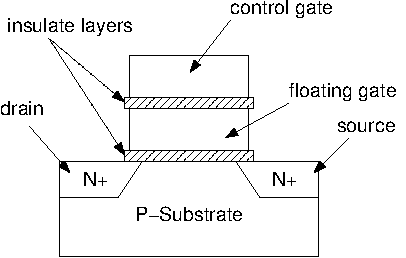
\includegraphics{cell}
\caption{schematic of a flash memory cell.\label{fig:cell}}
\end{figure} 

Because the floating gate is physically very close to the MOSFET
channel, even a small electric charge has an easily detectable effect on
the electrical behavior of the transistor. By applying appropriate
signals to the control gate and measuring the change in the transistor
behavior, it is therefore possible to determine whether or not there is
an electric charge on the floating gate.

Since the floating gate is electrically insulated from the rest of the
transistor, special techniques are required to move electrons to and
from it. One technique consists in filling the MOSFET channel with
high-energy electrons by applying relatively high voltages to the
control gate and the drain of the MOSFET. Some of these "hot" electrons
have sufficient energy to cross the barrier between the channel and the
floating gate. When the high voltages are removed, these electrons
remain trapped on the floating gate. This is the method used to program
a memory cell in EPROM and flash memories.

This technique, known as \emph{Channel Hot Electron} [CHE] injection,
can be used to load an electric charge onto the floating gate, but does
not provide a way to discharge it.  In order to discharge a floating
gate, flash memories\footnote{In EPROM memories, the floating gate is
  discharged by flooding the entire memory array with ultra-violet light
  --- the high-energy light penetrates the chip structure and impart
  enough energy to the trapped electrons, allowing them to escape the
  floating gate.}  tackle on a quantum effect known as \emph{tunneling}:
electrons are removed from the floating gate by applying a voltage to
the MOSFET that is large enough to cause electrons to 'tunnel' across
the insulating layer~\cite{Rajkanan:1996}.

Traditionally, the floating gate mechanism has been used to store a
single data bit, which is read by comparing the MOSFET threshold voltage
with a reference value.  More sophisticated techniques make it possible
to distinguish more than two floating gate charge states, thus enabling
two or more bits to be stored on a single floating gate. This is an
important technology breakthrough, because storing two bits/cell doubles
the memory capacity for a given cell size~\cite{intel-flash:2002}.


\section{Operation}

There are three basic operations that can be performed on a flash:
\emph{read}, \emph{program}, and \emph{erase}. Reading and programming a
flash is usually as fast as the equivalent operations on a DRAM (read
and write), but the erasing operation is much slower than reading or
programming.  This shortcoming is being tackled through partitioning and
also through the inclusion of pause operations that allow for operating
interweaving in a single partition.

The execution of these operations is managed and validated by the flash
own state-machine. Usually, the state-machine of a flash is also able to
detect operation time-outs, which may be an indicative of cell
degeneration.

\paragraph{Reading:}

reading from a flash memory is similar to reading from traditional
memory devices (e.g. DRAM). In order to reduce latency and improve
bandwidth, some flash memory units deploy sophisticate access modes:
besides traditional asynchronous bit and word read modes, they often
support asynchronous page read (buffering a whole page to speedup
subsequent accesses to the same page) and synchronous burst read
(multiple data words from a single address).

\paragraph{Programming:}

a typical flash memory is delivered with all sectors erased, i.e. with
all bits set to ``1''. Thus, programming (writing to) a flash consists
in turning some ``1s'' into ``0s''. Note that the reverse operation,
turning ``0s'' into ``1s'', is not defined\footnote{Trying to program a
  previously zeroed bit of a flash to ``1'' usually has no effect,
  though it probably causes the flash's state-machine to signalize a
  condition flag that might trigger external events.}. The only way to
set a bit in a flash is by erasing the whole sector. Some flash models
support programming single bits, words, and even blocks (burst write).
Some models also provide buffers to speed up programming, thus
supporting a write operating similar to DRAM (as long as one does not
try to overwrite a ``0'' with an ``1''). At transistor level, programing
a flash consists in injecting electrons into the floating gate.

\paragraph{Erasing:}

Erasing a sector of a flash memory unit, i.e. setting all of its bits to
``1'', is achieved by removing electrons from floating gates. Depending
on the technology used, a flash memory may be subjected to the so called
``over-erasing'' phenomenon: erasing a cell whose value is already ``1''
puts that cell in a state that prevents further programming. Flashes
exposed to the phenomenon usually handle it internally by programming
all bits of a sector (setting to ``0'') before erasing them (setting to
``1''). Therefore, erasing a flash becomes a trivial operation for
firmware/driver programmers.


%%%%%%%%%%%%%%%%%%%%%%%%%%%%%%%%%%%%%%%%%%%%%%%%%%%%%%%%%%%%%%%%%%%%%%%%
\chapter{Operating Systems and Flash Memory}

\emph{Flash memory} has been accepted as the industry ``de facto''
standard solution for non-volatile storage in embedded systems.
However, turning a "raw" flash memory chip into a usable
disk-replacement for embedded applications is a rather complex task.
This chapter discusses the use of flash memory in embedded systems from
the point of view of the operating system, including device drivers,
file systems, and update support.


\section{Device Drivers}

Some flash memory gadgets include additional components that emulate an
ordinary hard disk to the operating system. Such devices are usually
interfaced to a file system through a traditional hard disk device
driver that knows nothing about the peculiarities of flash memory
operation.  Nevertheless, ordinary flash memory units, as used in most
systems, do not include such additional disk-emulation logic. They rely
on specially designed device drivers to interface them to the file
subsystem's disk-like interface.

A \emph{flash memory device driver} differs from a RAM-disk driver in
that, besides mapping volume blocks into memory pages, it must also care
for an efficient management of flash memory limitations like sector
lifetime (for erasing), intra-sector rewriting of data, etc. Some device
drivers will handle flash particularities internally, exporting a
disk-like interface that supports the installation of an ordinary file
system on a flash memory device. A second approach would be to export an
interface with some flash-specific services. This second approach could
probably lead to a more effective flash usage, but it would also require
a flash-specific file system. Therefore, most systems opt for flash
device drivers that emulate an ordinary disk.


\subsection{Flash-specific Tasks}

Independently of the strategy chosen to export services, a flash driver
must handle several flash-specific tasks. The most important are
summarized in this section.

Traditional file systems are designed to update data in place. The same
disk sectors are constantly rewritten with new data.  This is a
reasonable mode of operation for magnetic media, but at odds with flash
memory, since there is a limitation in the number of times a flash can
be rewritten. Updating data in place on a flash would cause some sectors
(e.g. directories nodes) to expire their lifetimes far earlier than some
other sectors. Furthermore, today's typical flash sectors ($\sim$ 64
Kbytes) are too large to be directly mapped as disk blocks ($\sim$ 512
bytes).

There are two basic strategies to support the update of a small disk
block stored in a larger flash memory sector: erase-before-write and
remapping. The first strategy consists in coping the whole sector to a
temporary sector, erasing it, coping back unaltered blocks, and writing
the new contents of the block being updated to the proper offset in the
just-erased sector. The temporary sector must be subsequently erased.
The second strategy consists in having a translation table that maps
logical disk blocks in physical portions of flash sectors
(\emph{frames}). In this way, updating a block can be achieved by
writing the data into a new frame and updating the translation table.
Afterwards, the old frame is marked ``dead for posterior clean-up
procedures.

The remapping strategy has obvious performance advantages over immediate
rewriting. Besides, it allows for the homogeneous usage of sectors, so
the whole flash ages uniformly (\emph{wear-leveling}). However, it has
an important shortcoming: the need for \emph{garbage collection}.
Flagging frames as ``dead'' means leaving garbage behind in flash
sectors that must be later collected. Ideally, this operation would be
delayed until all frames in a sector are flagged ``dead'', so reclaiming
the sector (erasing it and putting it back at the free frame/sector
list) could be done without a single copy. In practice, however, it is
probable that many sectors will contain a mixture of dead and live
frames. In this case, live frames of a sector must be moved to other
sectors before its dead frames can be reclaimed.

Confronting remapping advantages (performance and wear-leveling) with
its disadvantages (garbage collection) usually leaves a positive result,
specially if the garbage collection procedure is implemented in such a
way that reclaiming is preventively performed in advance on flash's idle
time. Consequently, remapping became the most common approach to support
data update in flash memories.

Other flash-specific duties of device drivers are:

\begin{description}
  
\item[Data protection:] flash memory units often support write
  protecting individual sectors. This can be used to protect critical
  data such as bootstrap and operating system kernel.
  
\item[Fault recovery:] since most flash memory units do not implicitly
  validate write operations, a flash device driver must periodically
  check for data integrity.  If a failure is detected, the driver can
  mark the corresponding sector as ``bad'' and try to rewrite the data
  in other place. Write failures can be an indicative of life-time
  expiration.

\end{description}


\subsection{Case Studies}

At present time, there are many \emph{flash driver layers} available
both for commercial and open-source operating systems. The most
significant example of driver that supports windows-like file systems is
the proprietary \emph{Flash Translation Layer} [FTL], while the
\emph{Memory Technology Device} [MTD] driver is mostly adopted by
open-source systems. 
 
\paragraph{Flash Translation Layer [FTL]:}

FTL is a sector-based flash manager that provides logical to physical
sector mapping, thus enabling a flash to look like a disk to the
operating system~\cite{ftl}. As a rule, FTL supports any ordinary file
system to be installed on a flash, but it is mostly deployed with
windows-like systems such as VFAT.

\paragraph{Memory Technology Device [MTD]:}

MTD drivers are a new class of drivers developed under Linux
specifically for the embedded system area~\cite{mtd}. The main advantage
of MTD drivers over conventional block device drivers is that MTD
drivers are specifically designed for flash-based devices. Besides
exporting the typical \emph{raw block} interface for disk emulation, MTD
drivers also export a \emph{raw character} interface that allows file
systems to access the flash as if it were an ordinary linear memory
device.


\section{File Systems}

Application programs are able to store and retrieve data from flash
memory units through the services of a device driver. Very often,
however, the approach of directly controlling the storage of data
becomes inadequate, even in embedded system. If different applications
are to autonomously store data on the same flash memory, or if stored
data is intensively manipulated, then installing a \emph{file system}
will usually be a more effective approach.

Although the file system scene is a very rich one, few file systems have
being proposed for flash memory. This is mainly due to the fact that
most flash device drivers realize a disk-like interface that enables the
installation of non-flash-specific file systems on top of flash memory
units.  Nevertheless, a flash-specific file system will probably be
advantageous in regard to a disk file system, since it has the
opportunity to directly handle the limitations imposed by the
technology.


\subsection{Case Studies}

\paragraph{True Flash File System [TrueFFS]:}

M-Systems' TrueFFS~\cite{trueffs} implements the FTL standard and is
able to export the flash memory as a hard disk drive to the operating
system. It automatically handles wear-leveling, data protection, sector
mapping, garbage collection, and fault recovery. Though called a file
system, from a more strict point of view, TrueFFS would be considered a
flash device driver.  Indeed, TrueFFS requires the DOS FAT file system
on top of it.

\paragraph{Microsoft Flash File System [MFFS]:}

Microsoft's MFFS is a substratum for DOS FAT file systems.  Similarly to
the TrueFFS, it handles all traditional flash tasks. One of its
peculiarities is the adoption of variable size block, which can
optimizes garbage collection: a large segment of garbage in a block can
be converted into a new garbage-only block for immediate reuse.

\paragraph{Journalling Flash File System [JFFS]:}

Axis Communications' JFFS~\cite{jffs} differs from the traditional
``vitual disk'' approach used by TrueFFS and MFFS while implementing a
flash-specific file system for embedded systems. It was subsequently
extended by Red Hat, which distributes it as
JFFS2~\cite{Woodhouse:2001}. JFFS is a log-structured, compressing file
system~\cite{Rosenblum:1992} that is aware of the restrictions imposed
by flash memory and thus implements its operations in a more effective
way (through the \emph{raw character} interface of an MTD driver) .  For
instance, a log-rotating strategy executed periodically by the
garbage-collector also grants wear leveling. A JFFS file system could be
seen as a ``circular file'' that is written to the end, read from
anywhere, and erased (garbage collected) from the beginning.

\paragraph{Virtual File System [VFS]:}

PalmOS' VFS~\cite{vfs} requires the flash memory unit to be
encapsulated in a device that emulates an ordinary storage device and
therefore cannot be considered a flash file system. Nevertheless, it
implements a sort of lightweight database system that may be of interest
to some embedded applications.  VFS stores both programs and data as
collections of records that can be accessed via a database interface: a
rather convenient approach for \emph{Personal Information Manager}~[PIM]
applications.


\section{Update Support}

An apparently unimportant aspect of operating systems designed to
operate from/on flash memories is the way they can be updated, for the
time in which embedded systems were delivered with absolute, immutable
firmware is long gone. Today's embedded systems must consider regular
upgrade operations for firmware, operating system, and applications ---
the popular ``system reflashing''.

One aspect in which the operating system can easy or difficult updating
concerns the way it is stored in flash. If the system is a monolithic
piece of software installed on a predefined location in flash, it is
very likely the upgrading it will require the whole flash to be erased,
since the installation of a larger system image could corrupt
preexisting file system structures. Moreover, some systems are directly
executed from flash and allow applications to make absolute references
to internal functions. In this case, updating the system implies in
updating all applications. Such a condition could have serious
consequences for perpetual applications that store context information
in the flash.  For an example consider an \emph{odometer} application on
a car: reflashing the system without preserving the current mileage
count would transform an old chariot in a ``0 Km''. Typical Windows CE
installations present such shortcomings.

Reflashing side-effects can be avoided, or at least minimized, if the
operating system is itself installed in the file system. In this case,
upgrading the operating system solely requires some files to be
overwritten/added and has no direct effect on applications. Typical
Linux distributions for embedded systems function in this way. In
particular, the Familiar Linux distribution provides a tool called
``ipkg'' that is able to download packages from the network (via
``wget'') and install/upgrade them in a consistent way. Indeed, embedded
Linux distributions usually inherit on-the-fly upgrade mechanisms from
desktop distributions, like \emph{loadable kernel} modules and
\emph{dynamically linked libraries}.
 
\bibliography{flash}

\end{document}
